\documentclass[10pt]{beamer}

\usetheme[progressbar=foot]{metropolis}

\usepackage{booktabs} % Give nicer table (according to CTAN)
\usepackage{bm,graphicx,tabularx,array,booktabs,dcolumn,xcolor,microtype,multirow,amscd,amsmath,amssymb,amsfonts,physics,siunitx}
\usepackage[version=4]{mhchem}
\usepackage[utf8]{inputenc}
\usepackage[T1]{fontenc}
\usepackage{txfonts}
\usepackage[normalem]{ulem}
\usepackage{mleftright}
\usepackage{subcaption}

%============================================================%
%%% NEWCOMMANDS %%%
%============================================================%

%============================================================%
%%% NEWCOMMANDS %%%
% ============================================================%

%%% This latex gather all the latex commands that I use to facilitate the writing of electronic structure manuscript, report...
%%% You can import these commands by adding the following line in you .text
%%% %============================================================%
%%% NEWCOMMANDS %%%
% ============================================================%

%%% This latex gather all the latex commands that I use to facilitate the writing of electronic structure manuscript, report...
%%% You can import these commands by adding the following line in you .text
%%% %============================================================%
%%% NEWCOMMANDS %%%
% ============================================================%

%%% This latex gather all the latex commands that I use to facilitate the writing of electronic structure manuscript, report...
%%% You can import these commands by adding the following line in you .text
%%% \input{commands}

%%% Latin %%%

\newcommand{\ie}{\textit{i.e.}~}
\newcommand{\eg}{\textit{e.g.}~}
\newcommand{\etal}{\textit{et al.}~}

%%% Operators %%%

\newcommand{\hH}{\Hat{H}} % Hamiltonian operator
\newcommand{\HN}{\Hat{\mathnormal{H}}_{\text{N}}} % Normal ordered Hamiltonian
\newcommand{\Hsim}{\hat{\bar{H}}} % Similarity transformed Hamiltonian
\newcommand{\hC}{\Hat{C}} % CI operator
\newcommand{\hT}{\Hat{T}} % Cluster operator
\newcommand{\T}[1]{\Hat{\mathnormal{T}}_{#1}} % Cluster operator of a given excitation number
\newcommand{\hsig}{\Hat{\sigma}} % Unitary cluster operator
\newcommand{\hK}{\Hat{K}} % Anti-hermitian orbital rotation operator
\newcommand{\hS}{\Hat{S}} % Anti-hermitian CI coefficients rotation operator
\newcommand{\hP}[1]{\Hat{\mathnormal{P}}_{#1}} % Permutation operators

\newcommand{\hE}{\Hat{E}} % Spin averaged single excitation operator
\newcommand{\cre}[1]{a_{#1}^\dagger} % Creation operator
\newcommand{\ani}[1]{a_{#1}} % Annihilation operator
\newcommand{\bcre}[1]{b_{#1}^\dagger} % Boson creation operator
\newcommand{\bani}[1]{b_{#1}} % Boson annihilation operator

\newcommand{\com}[2]{\mleft[#1,#2 \mright]} % Commutator

%%% Wave functions %%%



%%% Matrix and tensor elements %%%

\newcommand{\oa}{O_{\alpha}}
\newcommand{\ob}{O_{\beta}}
\newcommand{\eri}[2]{\braket{#1}{#2}} % Electron repulsion integral physician notation
\newcommand{\ceri}[2]{\mleft(#1|#2\mright)} % Electron repulsion integral chemist notation
\newcommand{\dbi}[2]{\mel{#1}{}{#2}} % Double bar integral
\newcommand{\kron}[1]{\delta_{#1}} % Kronecker delta

%%% Matrix %%%

\newcommand{\FC}[1]{F_{#1}^{\text{C}}} % Core Fock matrix
\newcommand{\FA}[1]{F_{#1}^{\text{A}}} % Active Fock matrix

%%% Text acronyms and abbreviations %%%

\newcommand{\FCI}{\text{FCI}}
\newcommand{\HF}{\text{HF}}
\newcommand{\MCSCF}{\text{MCSCF}}
\newcommand{\occ}{\text{occ}}
\newcommand{\vir}{\text{vir}}


\newcommand{\SupInf}{\textcolor{blue}{Supporting Information}}



%%% Latin %%%

\newcommand{\ie}{\textit{i.e.}~}
\newcommand{\eg}{\textit{e.g.}~}
\newcommand{\etal}{\textit{et al.}~}

%%% Operators %%%

\newcommand{\hH}{\Hat{H}} % Hamiltonian operator
\newcommand{\HN}{\Hat{\mathnormal{H}}_{\text{N}}} % Normal ordered Hamiltonian
\newcommand{\Hsim}{\hat{\bar{H}}} % Similarity transformed Hamiltonian
\newcommand{\hC}{\Hat{C}} % CI operator
\newcommand{\hT}{\Hat{T}} % Cluster operator
\newcommand{\T}[1]{\Hat{\mathnormal{T}}_{#1}} % Cluster operator of a given excitation number
\newcommand{\hsig}{\Hat{\sigma}} % Unitary cluster operator
\newcommand{\hK}{\Hat{K}} % Anti-hermitian orbital rotation operator
\newcommand{\hS}{\Hat{S}} % Anti-hermitian CI coefficients rotation operator
\newcommand{\hP}[1]{\Hat{\mathnormal{P}}_{#1}} % Permutation operators

\newcommand{\hE}{\Hat{E}} % Spin averaged single excitation operator
\newcommand{\cre}[1]{a_{#1}^\dagger} % Creation operator
\newcommand{\ani}[1]{a_{#1}} % Annihilation operator
\newcommand{\bcre}[1]{b_{#1}^\dagger} % Boson creation operator
\newcommand{\bani}[1]{b_{#1}} % Boson annihilation operator

\newcommand{\com}[2]{\mleft[#1,#2 \mright]} % Commutator

%%% Wave functions %%%



%%% Matrix and tensor elements %%%

\newcommand{\oa}{O_{\alpha}}
\newcommand{\ob}{O_{\beta}}
\newcommand{\eri}[2]{\braket{#1}{#2}} % Electron repulsion integral physician notation
\newcommand{\ceri}[2]{\mleft(#1|#2\mright)} % Electron repulsion integral chemist notation
\newcommand{\dbi}[2]{\mel{#1}{}{#2}} % Double bar integral
\newcommand{\kron}[1]{\delta_{#1}} % Kronecker delta

%%% Matrix %%%

\newcommand{\FC}[1]{F_{#1}^{\text{C}}} % Core Fock matrix
\newcommand{\FA}[1]{F_{#1}^{\text{A}}} % Active Fock matrix

%%% Text acronyms and abbreviations %%%

\newcommand{\FCI}{\text{FCI}}
\newcommand{\HF}{\text{HF}}
\newcommand{\MCSCF}{\text{MCSCF}}
\newcommand{\occ}{\text{occ}}
\newcommand{\vir}{\text{vir}}


\newcommand{\SupInf}{\textcolor{blue}{Supporting Information}}



%%% Latin %%%

\newcommand{\ie}{\textit{i.e.}~}
\newcommand{\eg}{\textit{e.g.}~}
\newcommand{\etal}{\textit{et al.}~}

%%% Operators %%%

\newcommand{\hH}{\Hat{H}} % Hamiltonian operator
\newcommand{\HN}{\Hat{\mathnormal{H}}_{\text{N}}} % Normal ordered Hamiltonian
\newcommand{\Hsim}{\hat{\bar{H}}} % Similarity transformed Hamiltonian
\newcommand{\hC}{\Hat{C}} % CI operator
\newcommand{\hT}{\Hat{T}} % Cluster operator
\newcommand{\T}[1]{\Hat{\mathnormal{T}}_{#1}} % Cluster operator of a given excitation number
\newcommand{\hsig}{\Hat{\sigma}} % Unitary cluster operator
\newcommand{\hK}{\Hat{K}} % Anti-hermitian orbital rotation operator
\newcommand{\hS}{\Hat{S}} % Anti-hermitian CI coefficients rotation operator
\newcommand{\hP}[1]{\Hat{\mathnormal{P}}_{#1}} % Permutation operators

\newcommand{\hE}{\Hat{E}} % Spin averaged single excitation operator
\newcommand{\cre}[1]{a_{#1}^\dagger} % Creation operator
\newcommand{\ani}[1]{a_{#1}} % Annihilation operator
\newcommand{\bcre}[1]{b_{#1}^\dagger} % Boson creation operator
\newcommand{\bani}[1]{b_{#1}} % Boson annihilation operator

\newcommand{\com}[2]{\mleft[#1,#2 \mright]} % Commutator

%%% Wave functions %%%



%%% Matrix and tensor elements %%%

\newcommand{\oa}{O_{\alpha}}
\newcommand{\ob}{O_{\beta}}
\newcommand{\eri}[2]{\braket{#1}{#2}} % Electron repulsion integral physician notation
\newcommand{\ceri}[2]{\mleft(#1|#2\mright)} % Electron repulsion integral chemist notation
\newcommand{\dbi}[2]{\mel{#1}{}{#2}} % Double bar integral
\newcommand{\kron}[1]{\delta_{#1}} % Kronecker delta

%%% Matrix %%%

\newcommand{\FC}[1]{F_{#1}^{\text{C}}} % Core Fock matrix
\newcommand{\FA}[1]{F_{#1}^{\text{A}}} % Active Fock matrix

%%% Text acronyms and abbreviations %%%

\newcommand{\FCI}{\text{FCI}}
\newcommand{\HF}{\text{HF}}
\newcommand{\MCSCF}{\text{MCSCF}}
\newcommand{\occ}{\text{occ}}
\newcommand{\vir}{\text{vir}}


\newcommand{\SupInf}{\textcolor{blue}{Supporting Information}}



\usefonttheme[onlymath]{serif}

\makeatletter
\setlength{\metropolis@progressinheadfoot@linewidth}{2pt}
\setlength{\metropolis@titleseparator@linewidth}{2pt}
\setlength{\metropolis@progressonsectionpage@linewidth}{2pt}

\setbeamertemplate{title graphic}{
    \inserttitlegraphic
    \vspace{3mm}
}
\setbeamertemplate{title page}{
  \begin{minipage}[b][\paperheight]{\textwidth}
    \vfill
    \ifx\inserttitle\@empty\else\usebeamertemplate*{title}\fi
    \ifx\insertsubtitle\@empty\else\usebeamertemplate*{subtitle}\fi
    \usebeamertemplate*{title separator}
    \ifx\beamer@shortauthor\@empty\else\usebeamertemplate*{author}\fi
    \ifx\insertdate\@empty\else\usebeamertemplate*{date}\fi
    \ifx\insertinstitute\@empty\else\usebeamertemplate*{institute}\fi
    \vfill
    \ifx\inserttitlegraphic\@empty\else\usebeamertemplate*{title graphic}\fi
    \vspace*{1mm}
  \end{minipage}
}
\titlegraphic{\hfill
\includegraphics[height=1cm]{University_of_Oxford.pdf}\hspace{0.5cm}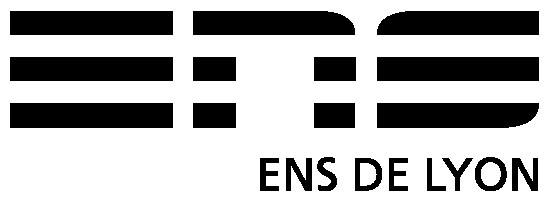
\includegraphics[height=1cm]{LogoENS.pdf}}

\setbeamertemplate{frame footer}{Insights on the CASSCF landscape}

\title{Understanding the CASSCF landscape:}
\subtitle{Towards a state-specific CASSCF algorithm?}
\date{\today}
\author{\textbf{Antoine Marie} \\
Supervised by Hugh Burton}
\institute{ENS de Lyon/University of Oxford}

\begin{document}

\maketitle

\section{The CASSCF theory}

\begin{frame}{The electronic problem}
  \metroset{block=fill}
  \pause[1]
  \begin{block}{The Shr\"odinger equation and its exact solution}
    \begin{equation}
      \hH \ket{\Psi} = E \ket{\Psi}
    \end{equation}

    \begin{equation}
      \label{eq:fci_wf}
      \ket{\Psi_{\FCI}} = \sum_I^{N_{det}} C_I\ket{I}
    \end{equation}
  \end{block}
  \pause[2]
  \begin{block}{One-electron basis}
    \begin{equation}
      \label{eq:MO}
      \phi_i(\bm{x}) = \sum^K_\mu c_i^\mu \chi_{\mu}(\bm{x})
    \end{equation}
  \end{block}
\end{frame}

\begin{frame}{The CASSCF ans\"atz}
  \metroset{block=fill}
  \pause[1]
  \begin{block}{The MCSCF ans\"atz}
    \begin{equation}
      \ket{\Psi}(\textcolor{red}{\bm{c}},\textcolor{red}{\bm{C}}) = \sum_I^{N_\text{trunc}} C_I\ket{I}
    \end{equation}
  \end{block}
  \pause[2]
  \begin{block}{The active space}
    \begin{equation*}
      \{\phi_i\} = \{\phi_i\}_{\text{core}}\cup \{\phi_i\}_{\text{act}}\cup \{\phi_i\}_{\text{vir}}
    \end{equation*}
    \begin{align}
      i \in \text{core} &\Rightarrow n_{\text{occ}}=2 \notag \\
      i \in \text{vir} &\Rightarrow n_{\text{occ}}=0 \notag \\
      i \in \text{act} &\Rightarrow n_{\text{occ}}=0,1~\text{or}~2 \notag
    \end{align}
  \end{block}
\end{frame}

\begin{frame}{Constraint-adapted ans\"atz}
  \metroset{block=fill}
  \pause[1]
  \begin{block}{Normalization constraints}
    \begin{align}
      \label{eq:constraint}
      \sum_I^N C^2_I &= 1 & \sum^K_\mu (c_i^\mu)^2 &= 1
    \end{align}
  \end{block}
  \pause[2]
  \begin{block}{MCSCF wave function}
    \begin{equation}
      \label{eq:mcscf_wf}
      \ket{\Psi_{\MCSCF}}(\textcolor{red}{\bm{\kappa}},\textcolor{red}{\bm{S}})=e^{\hK}e^{\hS}\ket{\Psi_0}
    \end{equation}
  \end{block}

  \begin{block}{Rotation operators}
    \begin{align}
      \hK &= \sum_{p,q} \kappa_p^q \left( \cre{q}\ani{p} - \cre{p}\ani{q} \right)  \\
      \hS &= \sum_{L \neq 0} S_{L}\left(\ket{\Psi_L}\bra{\Psi_0}-\ket{\Psi_0}\bra{\Psi_L}\right)
    \end{align}
  \end{block}

\end{frame}

\begin{frame}{The usual two-step process}
  \metroset{block=fill}
  \begin{figure}
    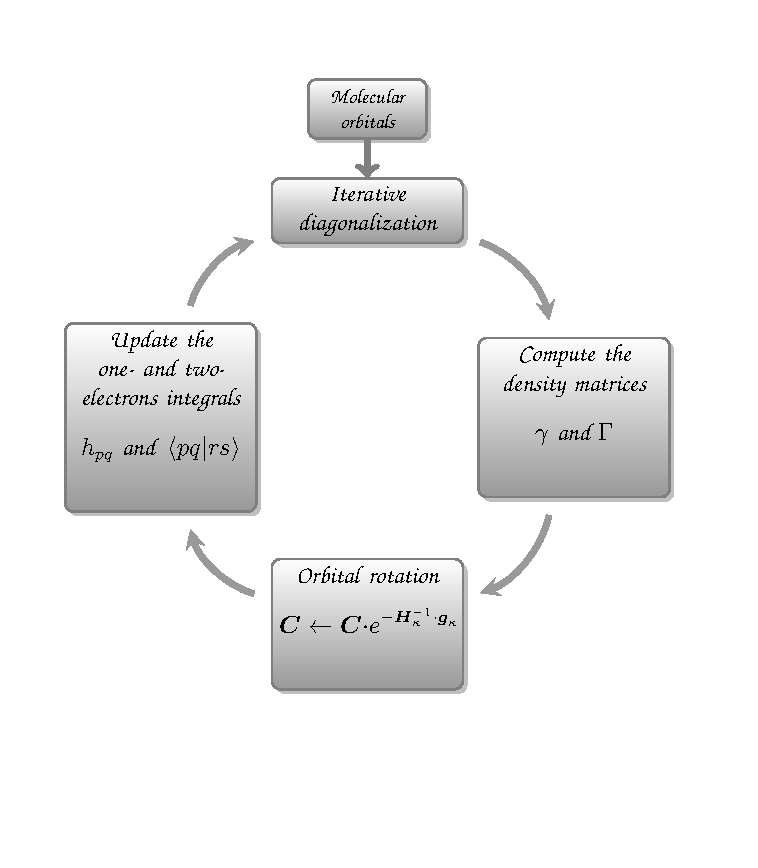
\includegraphics[width=0.7\textwidth]{two-step-process.pdf}
  \end{figure}
\end{frame}

\begin{frame}{State-average method for excited state}
  \metroset{block=fill}
  \pause[1]
  \begin{block}{State-averaged density matrices}
    \begin{align}
      \label{eq:sa_dm}
      \gamma_{\text{SA}} &= \sum_i^n w_i \gamma_i & \Gamma_{\text{SA}} &= \sum_i^n w_i \Gamma_i & \sum_i^n w_i&=1
    \end{align}
  \end{block}
  \pause[2]
  \begin{block}{Drawbacks of SA-CASSCF}
    \begin{itemize}
    \onslide<3,4,5> \item Limited to the states within the CAS
    \onslide<4,5> \item Need to compute lower excited states
    \onslide<5> \item Discontinuities
    \end{itemize}
  \end{block}
\end{frame}

\begin{frame}{One step Newton-Raphson process}
  \metroset{block=fill}
  \pause[1]
  \begin{block}{Taylor expansion}
    \begin{equation}
      \label{eq:MCSCF_NRJ_Taylor}
      E(\bm{\lambda}) = E(0) + \boldsymbol{g}^\dagger.\bm{\lambda} + \frac{1}{2} \bm{\lambda}^\dagger.\boldsymbol{H}.\bm{\lambda} + \dots,
    \end{equation}
  \end{block}
  \pause[2]
  \begin{block}{BCH expansion}
    \begin{equation}
      \label{eq:MCSCF_NRJ_BCH}
      \begin{split}
        E_{\text{MCSCF}} = &\mel{\Psi_0}{\hH}{\Psi_0} + \mel{\Psi_0}{[\hH,\hK]}{\Psi_0} + \mel{\Psi_0}{[\hH,\hS]}{\Psi_0}  \\
        &\frac{1}{2} \left(\mel{\Psi_0}{[[\hH,\hK],\hK]}{\Psi_0}+ \mel{\Psi_0}{[[\hH,\hS],\hS]}{\Psi_0}\right) \\
        &+ \mel{\Psi_0}{[[\hH,\hK],\hS]}{\Psi_0} + \dots
      \end{split}
    \end{equation}
  \end{block}
  \pause[3]
  \begin{block}{Newton-Raphson update}
    \begin{align}
      \bm{c}&= \bm{c}_0 e^{(-\bm{H}^{-1}\cdot \bm{g})_{\text{orb}}} & \bm{C}&= \bm{C}_0 e^{(-\bm{H}^{-1}\cdot \bm{g})_{\text{CI}}}
    \end{align}
  \end{block}
\end{frame}

\begin{frame}{Distinguishing solutions}
  \metroset{block=fill}
  \begin{block}{Generalized Fock matrix}
    \begin{equation}
      \label{eq:general_fock}
      F_{xy} = \sum_q \gamma_{xq}h_{yq} + \sum_{qrs} \Gamma_{xqrs}\ceri{yq}{rs}
    \end{equation}
  \end{block}
\end{frame}

\section{Test case: the hydrogen molecule}

\begin{frame}{Proof of principle: \ce{H2} STO-3G}

  \begin{figure}
    \centering

    \begin{columns}

      \begin{column}{0.15\textwidth}
        
        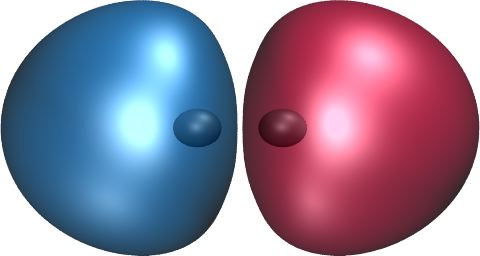
\includegraphics[width=0.9\textwidth]{Figures/H2_SA_mo1.cube.png}
        \caption*{\centering $n_\text{occ}~=~0.012$
        $\sigma_u$}
        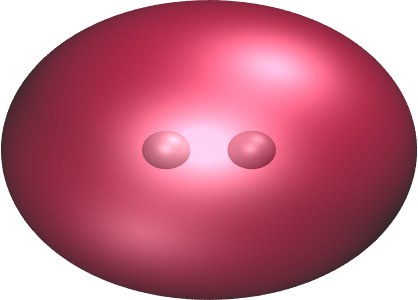
\includegraphics[width=0.9\textwidth]{Figures/H2_SA_mo2.cube.png}
        \caption*{\centering $n_\text{occ}~=~1.988$
        $\sigma_g$}
      \end{column}

      \begin{column}{0.68\textwidth}
        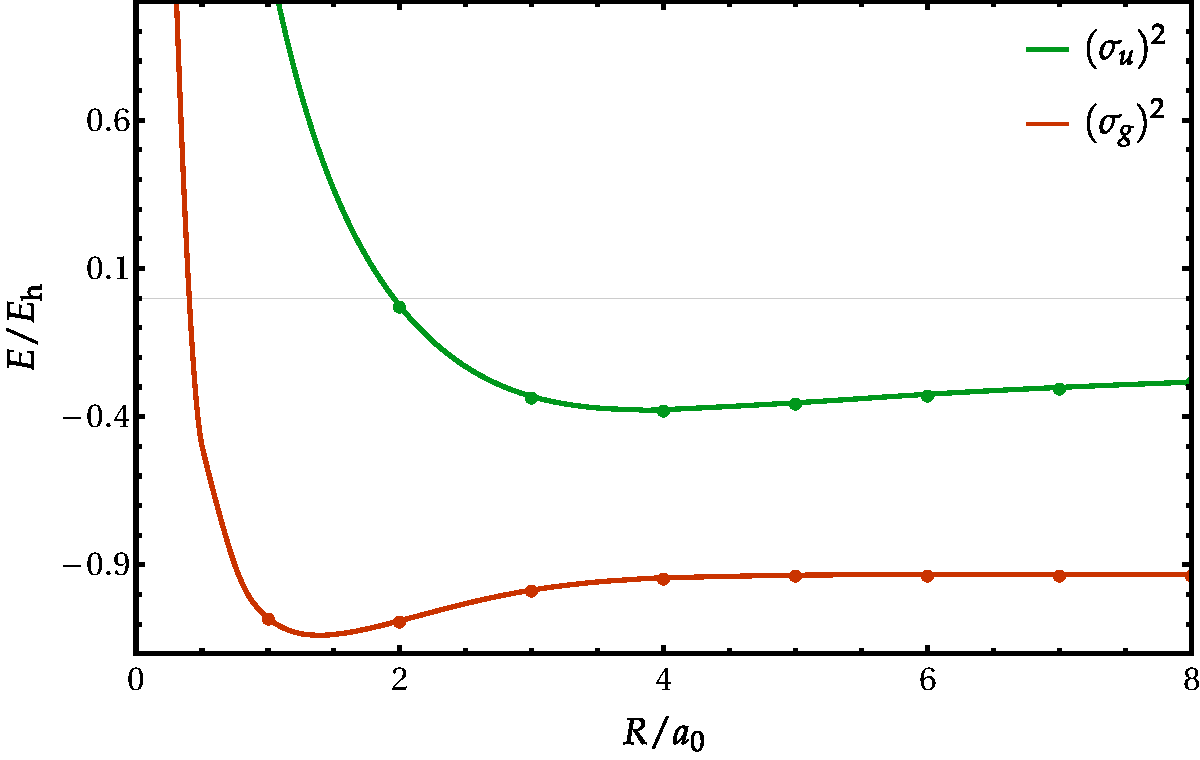
\includegraphics[width=0.9\textwidth]{Figures/fig_1a.pdf}
      \end{column}

      \begin{column}{0.15\textwidth}
        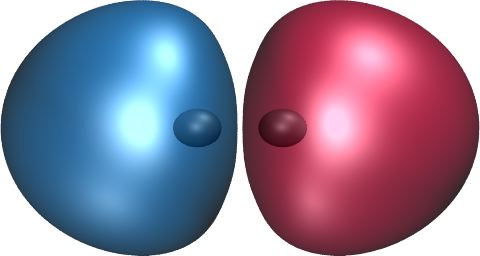
\includegraphics[width=0.9\textwidth]{Figures/H2_SA_mo1.cube.png}
        \caption*{\centering $n_\text{occ}~=~1.988$
        $\sigma_u$}
        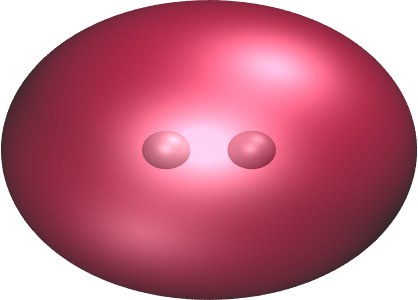
\includegraphics[width=0.9\textwidth]{Figures/H2_SA_mo2.cube.png}
        \caption*{\centering $n_\text{occ}~=~0.012$
        $\sigma_g$}
      \end{column}
      
    \end{columns}

    % \caption{
    % CID energies of \ce{H_2} in the STO-3G basis set with respect to the bond length $R$. The crosses represent the corresponding FCI energies.
    % \label{fig:fig_1}}
  \end{figure}
  
\end{frame}

\begin{frame}{Proof of principle: \ce{H2} STO-3G}

  \begin{figure}
    \centering

    \begin{columns}

      \begin{column}{0.15\textwidth}
        
        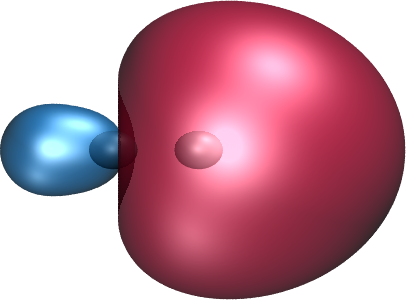
\includegraphics[width=0.9\textwidth]{Figures/H2_SB1_mo1.cube.png}
        \caption*{\centering $n_\text{occ}~=~1.000$
        $\sigma_u$}
        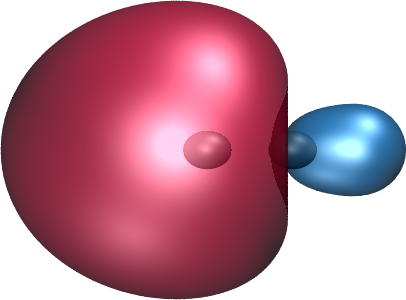
\includegraphics[width=0.9\textwidth]{Figures/H2_SB1_mo2.cube.png}
        \caption*{\centering $n_\text{occ}~=~1.000$
        $\sigma_g$}
      \end{column}

      \begin{column}{0.68\textwidth}
        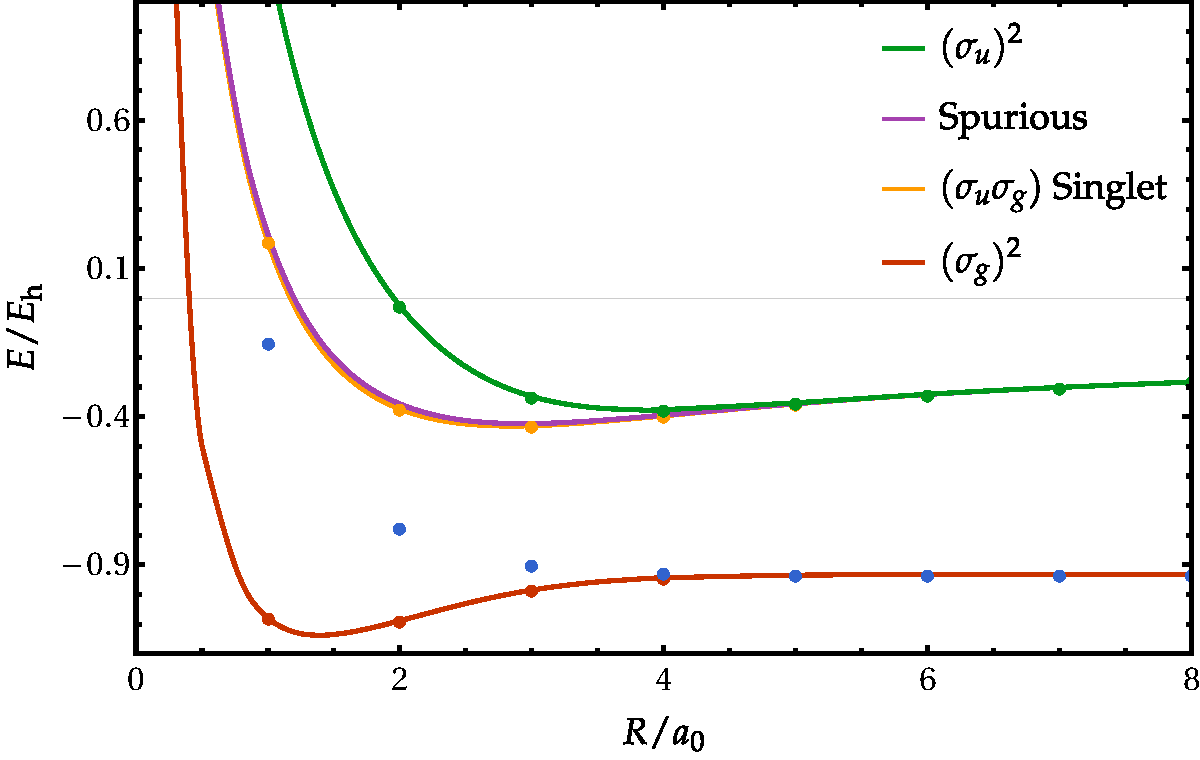
\includegraphics[width=0.9\textwidth]{Figures/fig_1b.pdf}
      \end{column}

      \begin{column}{0.15\textwidth}
        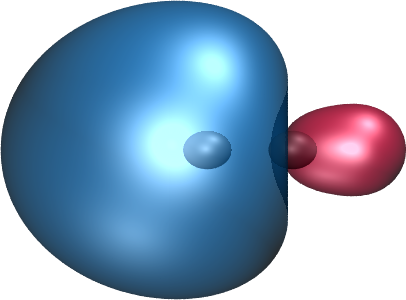
\includegraphics[width=0.9\textwidth]{Figures/H2_SB2_mo1.cube.png}
        \caption*{\centering $n_\text{occ}~=~1.000$
        $\sigma_u$}
        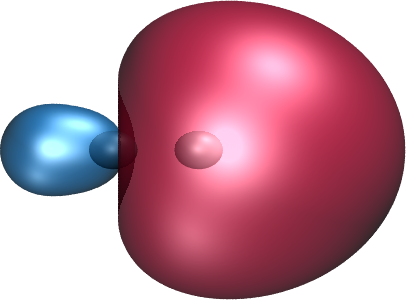
\includegraphics[width=0.9\textwidth]{Figures/H2_SB2_mo2.cube.png}
        \caption*{\centering $n_\text{occ}~=~1.000$
        $\sigma_g$}
      \end{column}
      
    \end{columns}

    % \caption{
    % oo-CID energies of \ce{H_2} in the STO-3G basis set with respect to the bond length $R$. The crosses represent the corresponding FCI energies.
    % \label{fig:fig_2}}
  \end{figure}
  
\end{frame}

\begin{frame}{\ce{H2} 6-31G $R=1~a_0$: Triplet states}
  \begin{table}
    \label{tab:tab_1}
    \begin{tabular}{ccccc}
      state & FCI  & SA(2,2) & SA(3,2) & SS(2,2) \\
      \hline
      \onslide<1,2,3,4>1 & -0.57616 & \onslide<2,3,4>-0.57166 & \onslide<3,4>-0.57406 & \onslide<4>-0.57417 \\
      \onslide<1,2,3,4>2 & -0.28180 &  & \onslide<3,4>-0.27990 & \onslide<4>-0.27990 \\
      \onslide<1,2,3,4>3 & 0.51519 &  & \onslide<3,4>0.51654 & \onslide<4>0.51638 \\
      \onslide<1,2,3,4>4 & 0.62520 &  &  & \onslide<4>0.62401 \\
      \onslide<1,2,3,4>5 & 1.30761 &  &  & \onslide<4>1.30572 \\
      \onslide<1,2,3,4>6 & 1.61884 &  &  & \onslide<4>1.61685 \\
    \end{tabular}
  \end{table}
\end{frame}

\begin{frame}{\ce{H2} 6-31G $R=1~a_0$: Singlet states}
  \begin{table}
    \label{tab:tab_2}
    \begin{tabular}{ccccc}
       state & FCI  & SA(2,2) & SA(3,2) & SS(2,2) \\
      \hline
      1 & -1.09897 & -1.07170 & -1.08924 & -1.09225 \\
      2 & -0.46395 & -0.43494 & -0.44196 & -0.46368 \\
      3 & -0.07450 &  & -0.06164 & -0.0594551 \\
      4 & 0.32015 & 0.33066 & 0.32624 & 0.31914 \\
      5 & 0.57224 &  & 0.61682 & 0.61429 \\
      6 & 0.86353 &  & 0.86876 & 0.86392 \\
      7 & 0.96373 &  &  & 0.91147 \\
      8 & 1.46479 &  &  & 1.45704 \\
      9 & 1.81277 &  &  & 1.80747 \\
      10 & 2.71948 &  &  & 2.71766 \\
    \end{tabular}
  \end{table}
\end{frame}

\begin{frame}{\ce{H2} 6-31G $R=1~a_0$: Spurious states}
  \begin{table}
    \label{tab:tab_3}
    \begin{tabular}{ccccc}
      state & FCI  & SA(2,2) & SA(3,2) & SS(2,2) \\
      \hline
      1 & -1.09897 & -1.07170 & -1.08924 & -1.09225 \\
      Spurious &  &  &  & -1.08569 \\
      Spurious &  &  &  & -1.07871 \\
      \hline
      4 & 0.32015 & 0.33066 & 0.32624 & 0.31914 \\
      Spurious &  &  &  & 0.31821 \\
      Spurious &  &  &  & 0.31844 \\
      Spurious &  &  &  & 0.32440 \\
      \hline
      6 & 0.86353 &  & 0.86876 & 0.86392 \\
      Spurious &  &  &  & 0.85673 \\
      Spurious &  &  &  & 0.86266 \\
      Spurious &  &  &  & 0.86266 \\
      \hline
      10 & 2.71948 &  &  & 2.71766 \\
      Spurious &  &  &  & 2.70046 \\
      Spurious &  &  &  & 2.69883 \\
    \end{tabular}
  \end{table}
\end{frame}

\section{Understanding the spurious solutions}

\begin{frame}{Influence of the basis set: \ce{H2} $R=1~a_0$}
  \begin{figure}
    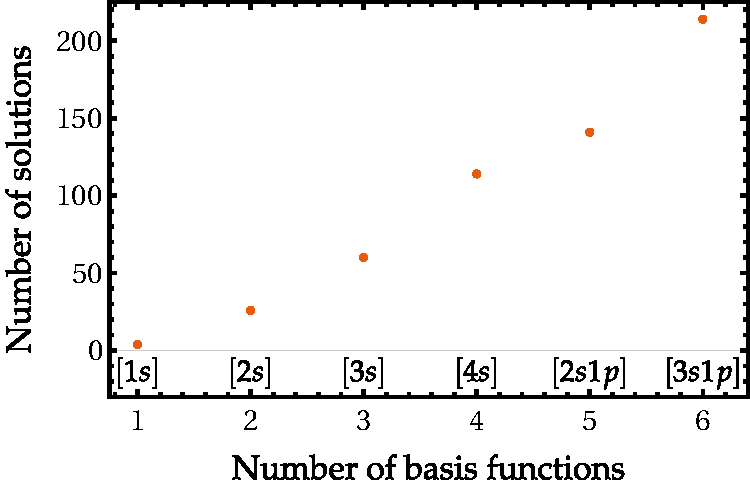
\includegraphics[width=0.8\textwidth]{Figures/fig_3a.pdf}
  \end{figure}
\end{frame}

\begin{frame}{Influence of frozen orbitals: \ce{HF} STO-3G $R=2~a_0$}
  \begin{figure}
    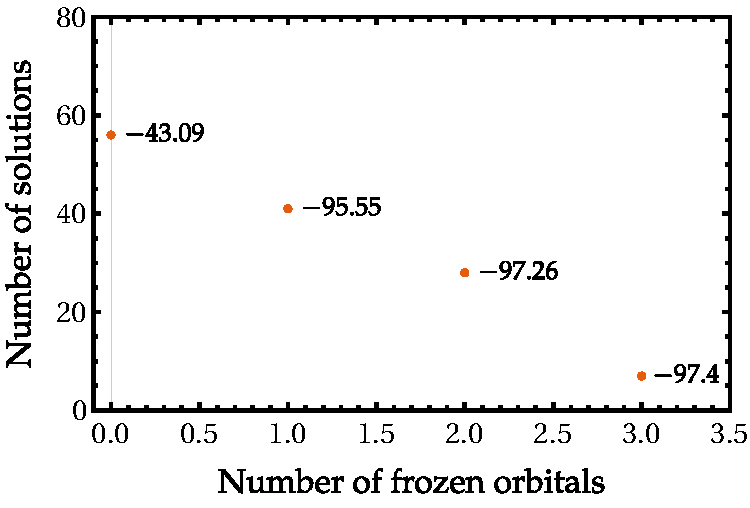
\includegraphics[width=0.8\textwidth]{Figures/fig_3b.pdf}
  \end{figure}
\end{frame}

\begin{frame}{Influence of the bond length: \ce{H2} 6-31G}
  \begin{figure}
    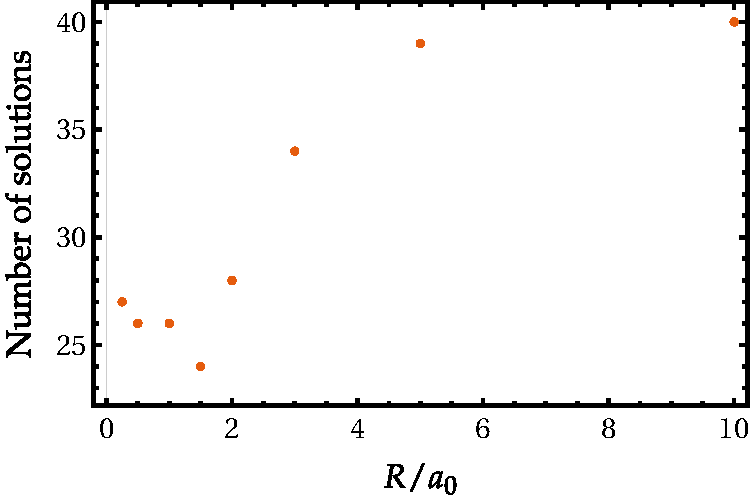
\includegraphics[width=0.8\textwidth]{Figures/fig_3c.pdf}
  \end{figure}
\end{frame}

\begin{frame}{Index of the solutions: \ce{H2} 6-31G}

  \begin{figure}
    \begin{columns}
      
      \pause[1]
      \begin{column}{0.48\textwidth}
        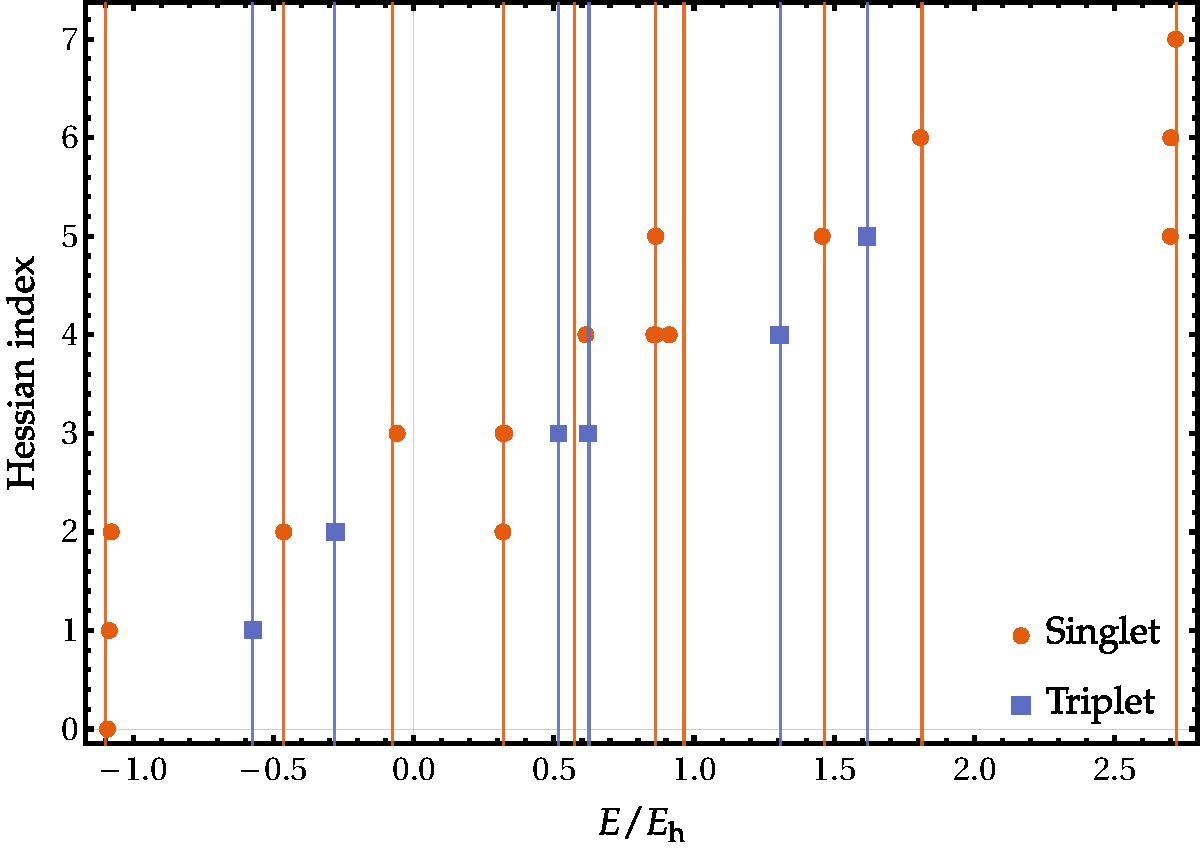
\includegraphics[width=\textwidth]{Figures/fig_2a.pdf}
      \end{column}

      \pause[2]
      \begin{column}{0.48\textwidth}
        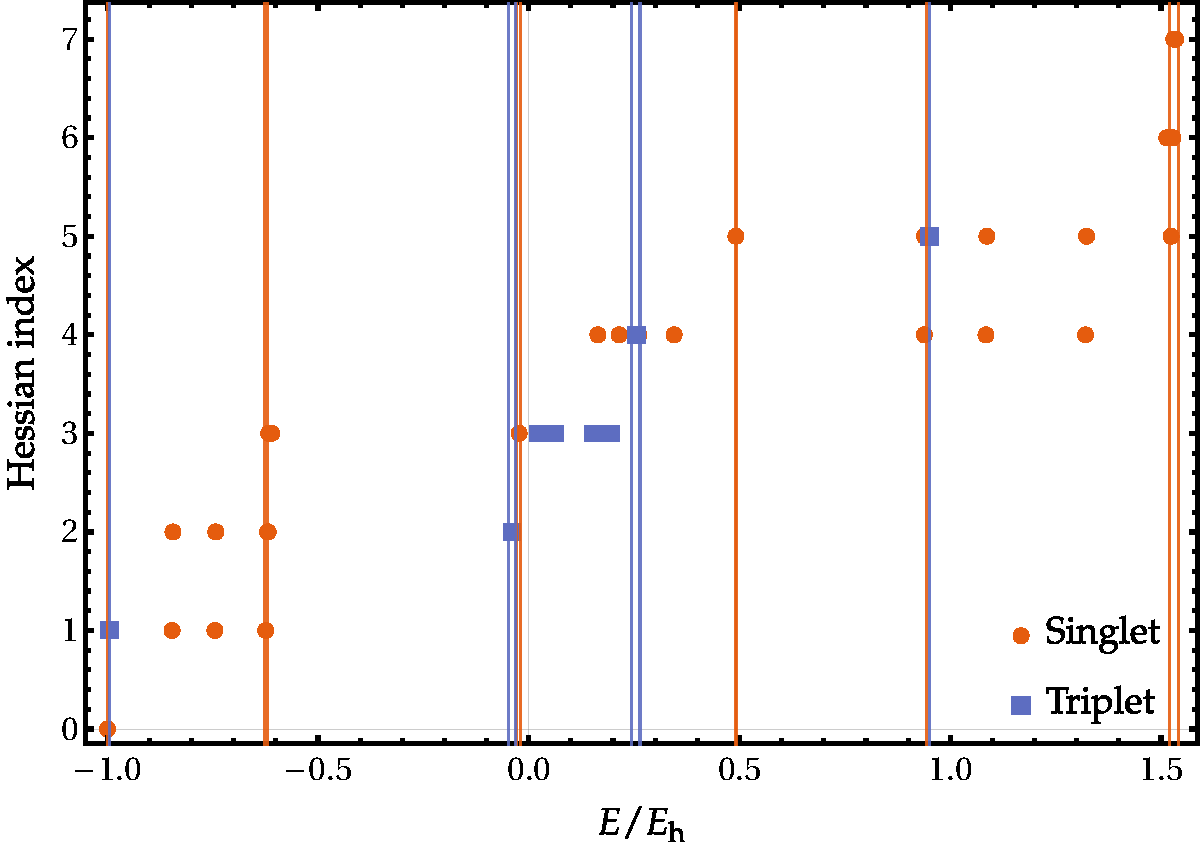
\includegraphics[width=\textwidth]{Figures/fig_2b.pdf}
      \end{column}
      
    \end{columns}

    % \caption{Index of the (2,2) SS-CASSCF solutions with respect to their energy. Left: $R=1~a_0$. Right: $R=5~a_0$.}
  \end{figure}
  
\end{frame}

\begin{frame}{Ground-state potential energy surface: \ce{H2} 6-31g}
  \begin{figure}
    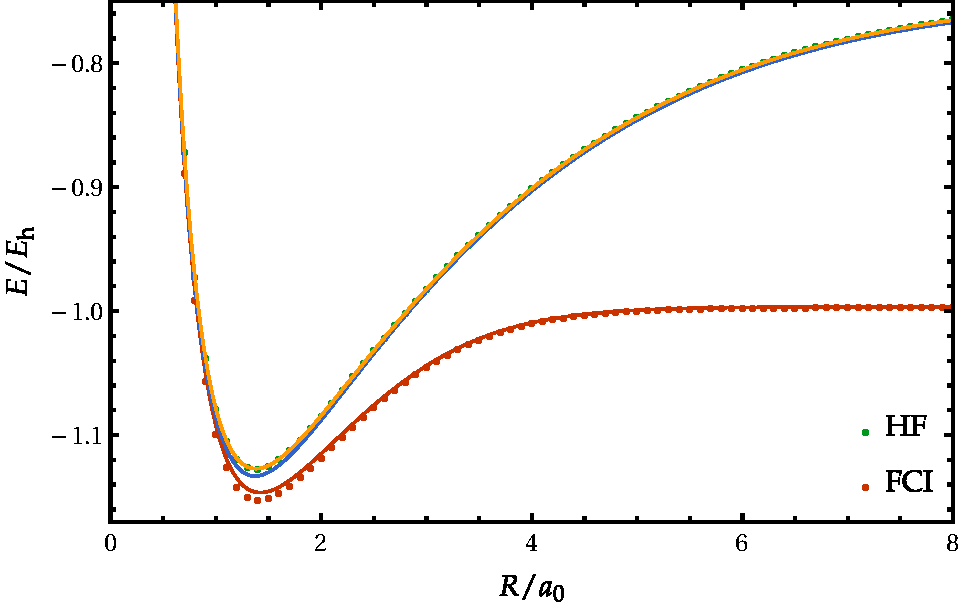
\includegraphics[width=0.9\textwidth]{Figures/fig_4.pdf}
    % \caption{PES of the three lowest (2,2) SS-CASSCF solutions. The dots represent the corresponding HF and FCI states.}
  \end{figure}
\end{frame}

\begin{frame}{Natural orbitals of the ground-state solutions: \ce{H2} 6-31g $R=1~a_0$}
  \begin{figure}
    \begin{columns}[b]
      \pause[1]
      \begin{column}{0.31\textwidth}
        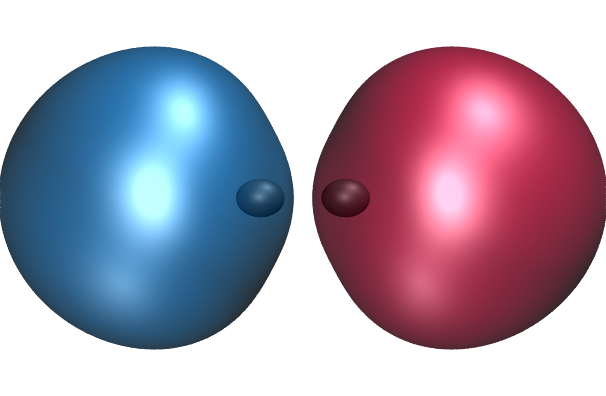
\includegraphics[width=0.7\textwidth]{Figures/h2_HF_mo2.cube.png}
        \caption*{\centering $(1\sigma_u)~n_\text{occ}~=~0.011$}
        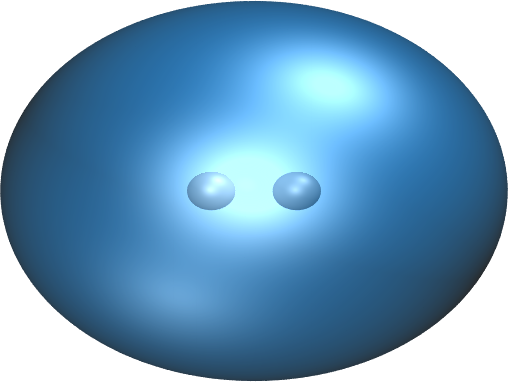
\includegraphics[width=0.7\textwidth]{Figures/h2_HF_mo1.cube.png}
        \caption*{\centering $(1\sigma_g)~n_\text{occ}~=~1.989$
        $E=-1.09225~E_h$}
      \end{column}
      \pause[2]
      \begin{column}{0.31\textwidth}
        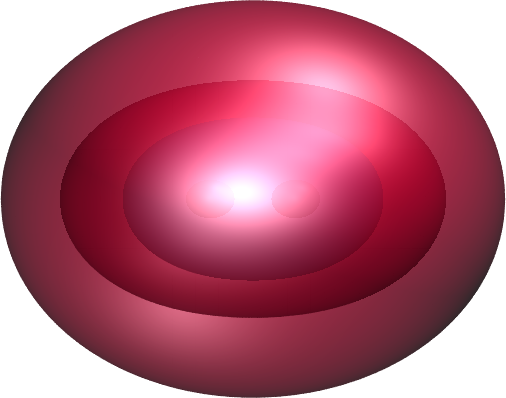
\includegraphics[width=0.7\textwidth]{Figures/h2_HF_mo3.cube.png}
        \caption*{\centering $(2\sigma_g)~n_\text{occ}~=~0.007$}
        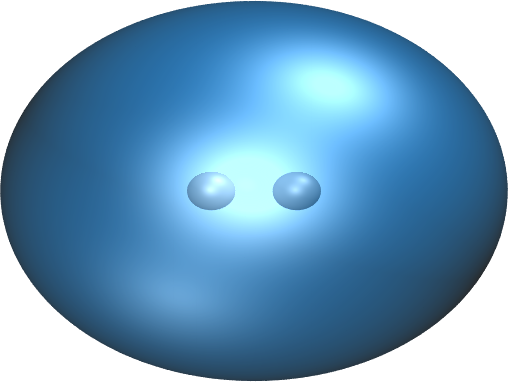
\includegraphics[width=0.7\textwidth]{Figures/h2_HF_mo1.cube.png}
        \caption*{\centering $(1\sigma_g)~n_\text{occ}~=~1.993$
        $E=-1.08569~E_h$}
      \end{column}
      \pause[3]
      \begin{column}{0.31\textwidth}
        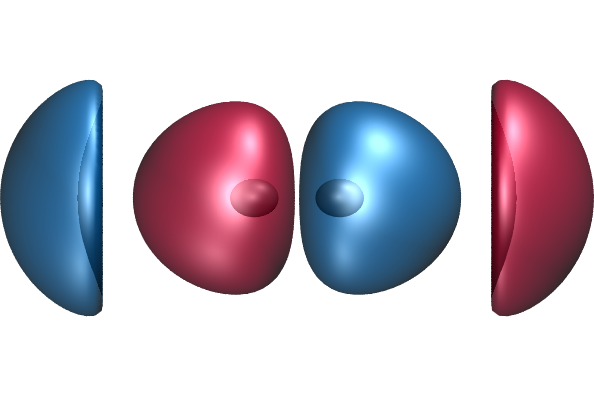
\includegraphics[width=0.7\textwidth]{Figures/h2_HF_mo4.cube.png}
        \caption*{\centering $(2\sigma_u)~n_\text{occ}~=~0.0002$}
        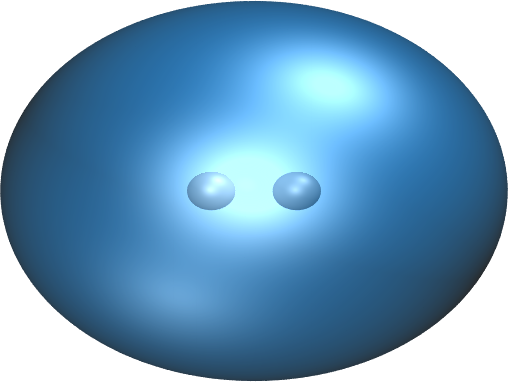
\includegraphics[width=0.7\textwidth]{Figures/h2_HF_mo1.cube.png}
        \caption*{\centering $(1\sigma_g)~n_\text{occ}~=~1.9998$
        $E=-1.07871~E_h$}
      \end{column}
      
    \end{columns}
  \end{figure}
\end{frame}

\begin{frame}{Natural orbitals of the ground-state solutions: \ce{H2} 6-31g $R=8~a_0$}
  \begin{figure}
    \begin{columns}[b]

      \begin{column}{0.31\textwidth}
        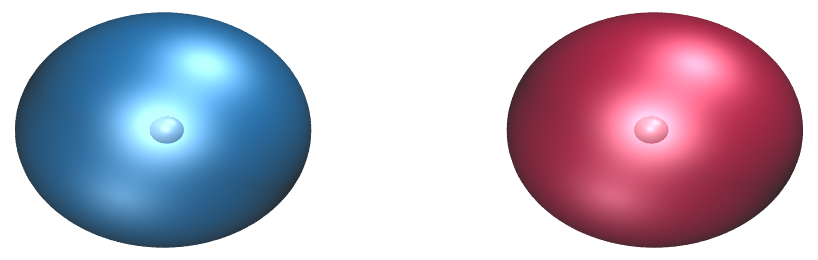
\includegraphics[width=0.7\textwidth]{Figures/h2_r8_HF_mo2.cube.png}
        \caption*{\centering $(1\sigma_u)~n_\text{occ}~=~0.985$}
        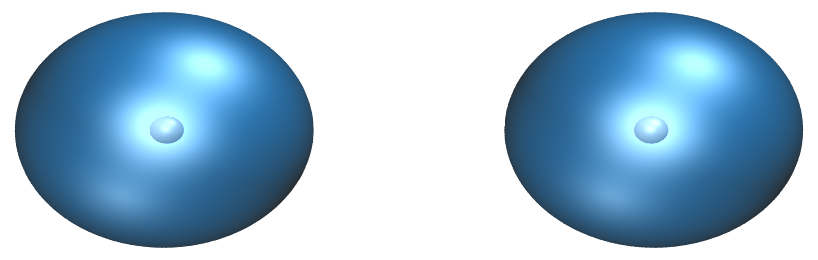
\includegraphics[width=0.7\textwidth]{Figures/h2_r8_HF_mo1.cube.png}
        \caption*{\centering $(1\sigma_g)~n_\text{occ}~=~1.015$
          $E=0.996485~E_h$}
      \end{column}
    
      \begin{column}{0.31\textwidth}
        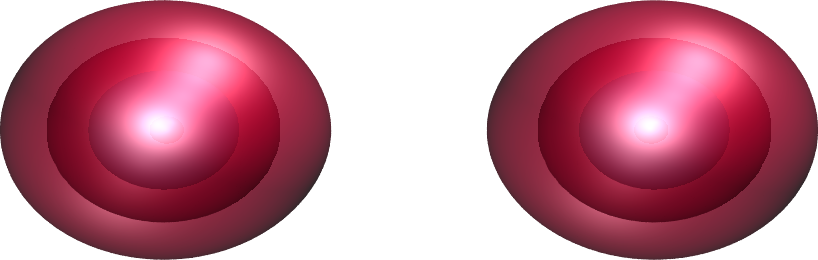
\includegraphics[width=0.7\textwidth]{Figures/h2_r8_HF_mo3.cube.png}
        \caption*{\centering $(2\sigma_g)~n_\text{occ}~=~0.003$}
        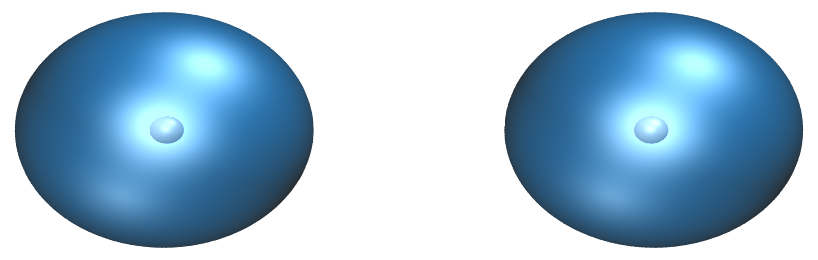
\includegraphics[width=0.7\textwidth]{Figures/h2_r8_HF_mo1.cube.png}
        \caption*{\centering $(1\sigma_g)~n_\text{occ}~=~1.997$
          $E=-0.767073~E_h$}
      \end{column}
    
      \begin{column}{0.31\textwidth}
        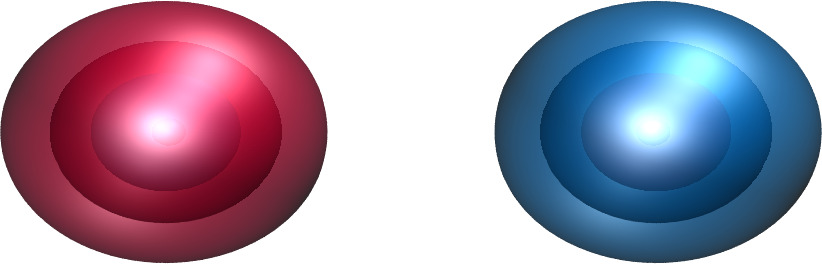
\includegraphics[width=0.7\textwidth]{Figures/h2_r8_HF_mo4.cube.png}
        \caption*{\centering $(2\sigma_u)~n_\text{occ}~=~0.001$}
        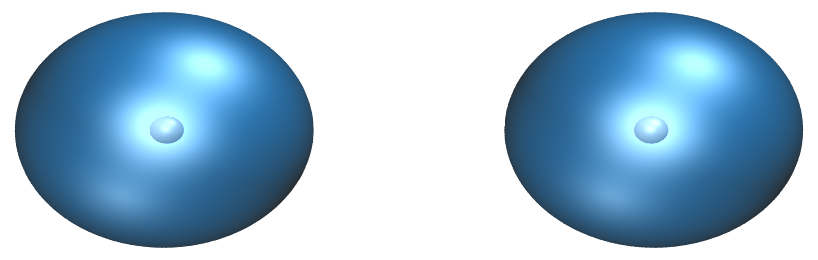
\includegraphics[width=0.7\textwidth]{Figures/h2_r8_HF_mo1.cube.png}
        \caption*{\centering $(1\sigma_g)~n_\text{occ}~=~1.999$
          $E=-0.764297~E_h$}
      \end{column}
    
    \end{columns}
  \end{figure} 
\end{frame}

\begin{frame}{Triplet states potential energy surfaces: \ce{H2} 6-31G}
  \begin{figure}
    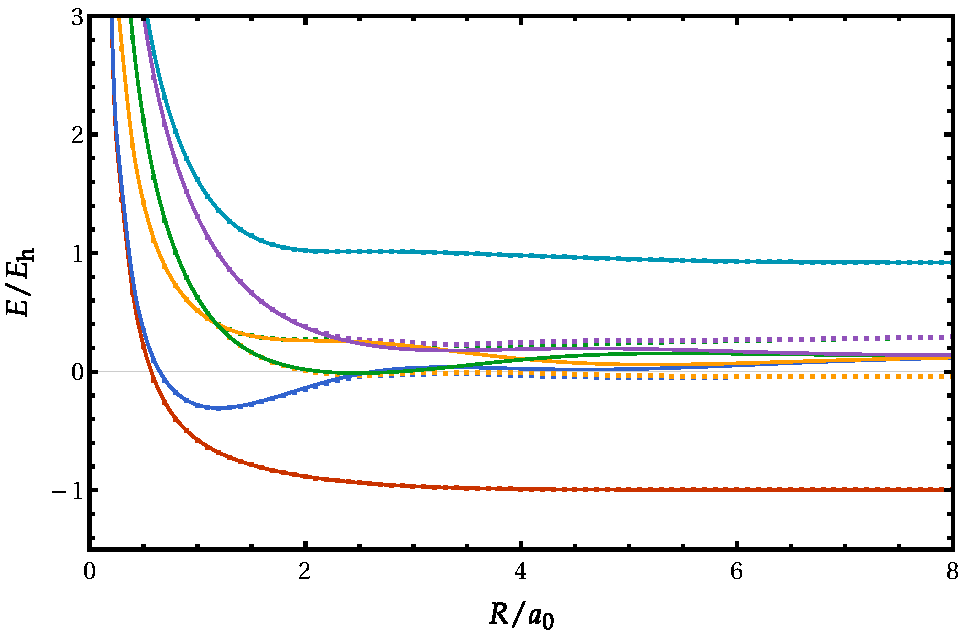
\includegraphics[width=0.9\textwidth]{Figures/fig_6a.pdf}
    % \caption{PES of the six triplet (2,2) SS-CASSCF solutions. The dots represent the corresponding HF and FCI states.}
  \end{figure}
\end{frame}

\begin{frame}{CASSCF Coulson-Fisher points}
  \begin{figure}
    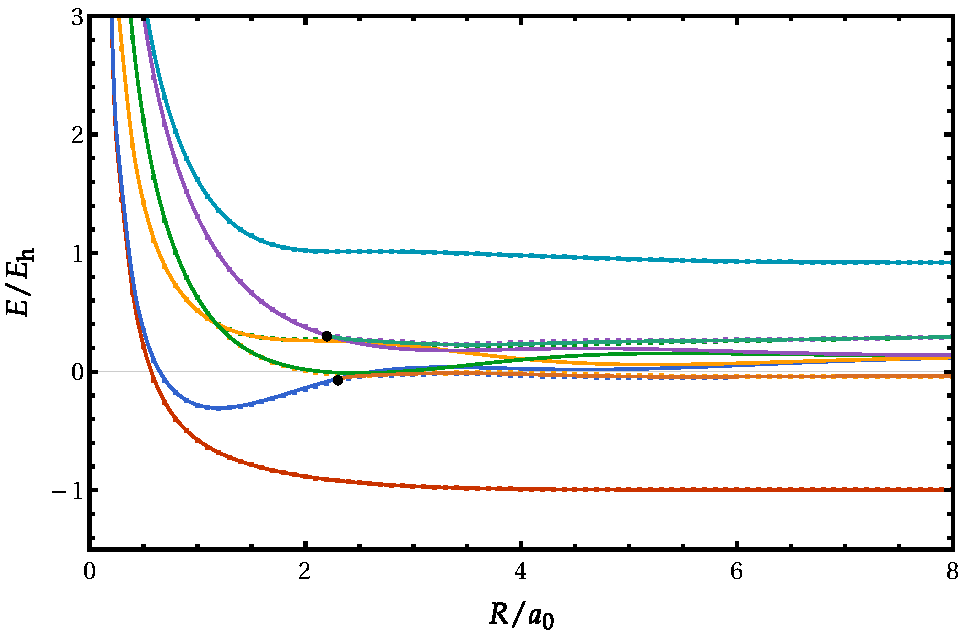
\includegraphics[width=0.9\textwidth]{Figures/fig_6b.pdf}
    % \caption{PES of the triplet (2,2) SS-CASSCF solutions. The dots represent the corresponding HF and FCI states.}
  \end{figure}
\end{frame}

\begin{frame}{Open-shell singlet potential energy surfaces: \ce{H2} 6-31G}
  \begin{figure}
    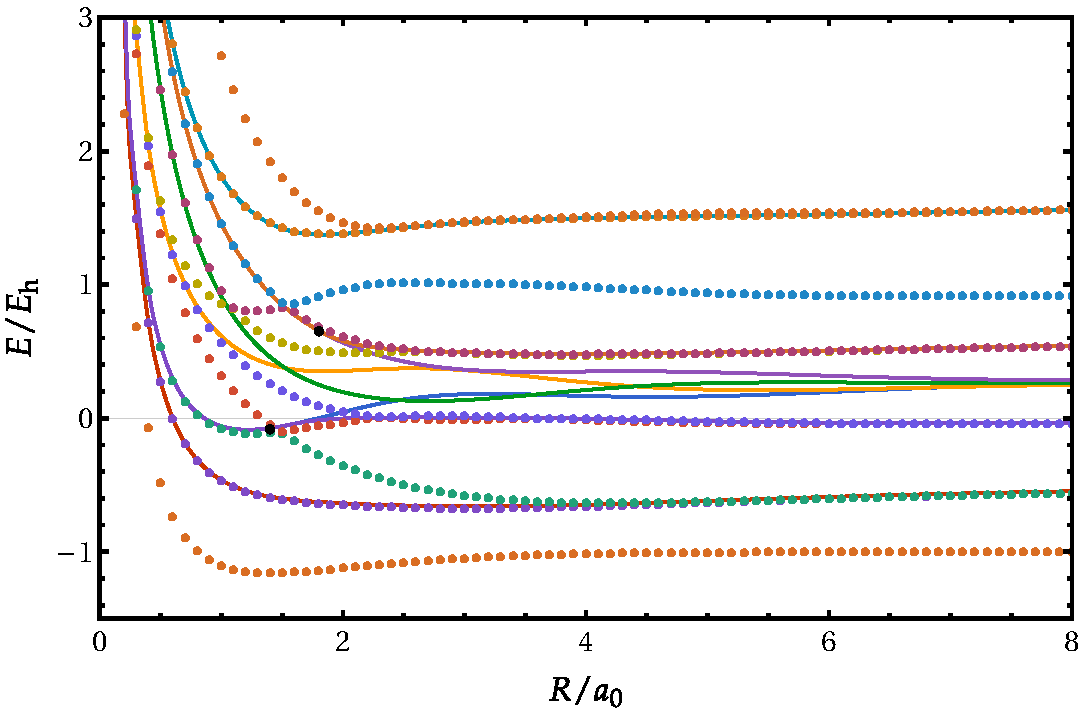
\includegraphics[width=0.9\textwidth]{Figures/fig_7a.pdf}
    % \caption{PES of the six open-shell (2,2) SS-CASSCF solutions. The dots represent the corresponding HF and FCI states.}
  \end{figure}
\end{frame}

\begin{frame}{Closed-shell singlet potential energy surfaces: \ce{H2} 6-31G}
  \begin{figure}
    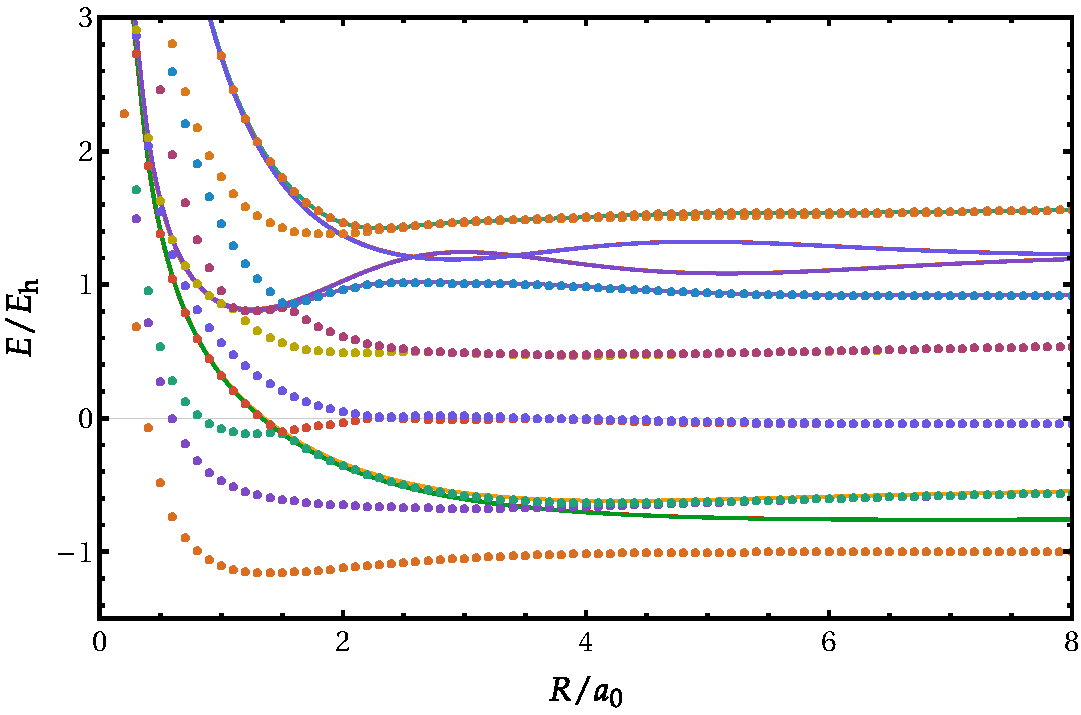
\includegraphics[width=0.9\textwidth]{Figures/fig_7b.pdf}
    % \caption{PES of the six open-shell (2,2) SS-CASSCF solutions. The dots represent the corresponding HF and FCI states.}
  \end{figure}
\end{frame}

\begin{frame}{Influence of the basis set: \onslide<2>{\ce{H2} 6-311G $R=1~a_0$}}
  \pause[1]
  \begin{figure}
    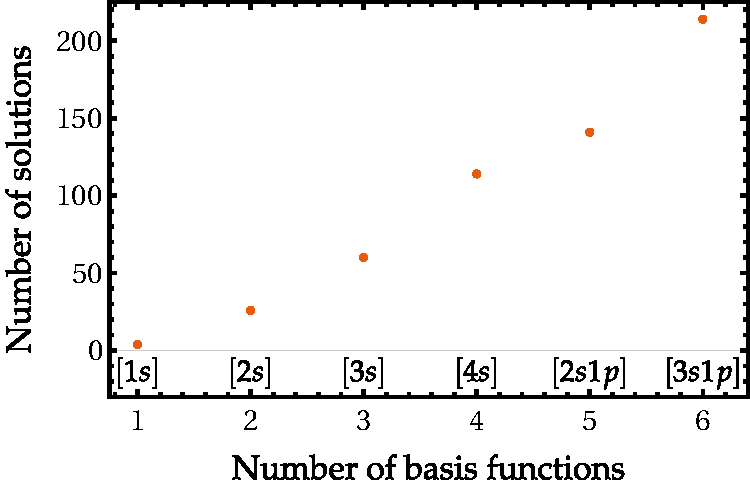
\includegraphics[width=0.8\textwidth]{Figures/fig_3a.pdf}
  \end{figure}
  \pause[2]
  \begin{table}
    \label{tab:tab_4}
    \begin{tabular}{clllll}
      FCI & -1.10267 & & & &\\
      \hline
      SS(2,2) & -1.09429 & -1.08866 & -1.08074 & -1.08033 & -1.08026 \\
    \end{tabular}
  \end{table}
\end{frame}

\begin{frame}{Influence of the CAS: \ce{H2} 6-31G $R=1~a_0$}
  \begin{table}
    \label{tab:tab_5}
    \begin{tabular}{cllll}
      \pause[1]
      state & 1  & 2 & 3 & 4 \\
      \hline
      FCI & -1.09897 & -0.46395 & -0.07450 & 0.32015 \\
      \hline
      SS(2,2) & -1.09225 & -0.46368 & -0.0594551 & 0.31914 \\
            & -1.08569 &  &  & 0.31821 \\
            & -1.07871 &  &  & 0.31844 \\
            &  &  &  & 0.32440 \\
      \hline
      \pause[2]
      SS(3,2) & -1.09875 & \onslide<4>{-0.463822} & \onslide<4>{-0.0711398} & \onslide<3,4>{0.315896} \\
            & -1.09256 & \onslide<4>{-0.463689} & \onslide<4>{-0.0632185} & \onslide<3,4>{0.320249} \\
            & -1.08581 &  & \onslide<4>{-0.0594551} & \onslide<3,4>{0.322577} \\
    \end{tabular}
  \end{table}
\end{frame}

\section{Avoided crossings}

\begin{frame}{Weak avoided crossing: \ce{LiH} STO-3G}
  \begin{figure}
    \includegraphics<1>[width=0.9\textwidth]{Figures/fig_8a.pdf}
    \includegraphics<2>[width=0.9\textwidth]{Figures/fig_8b.pdf}
    % \caption{PES of the six lowest states of LiH in the STO-3G basis set.}
  \end{figure}
\end{frame}

\begin{frame}{Strong avoided crossing: \ce{LiF} STO-3G}
  \begin{figure}
    \includegraphics<1>[width=0.9\textwidth]{Figures/fig_9a.pdf}
    \includegraphics<2>[width=0.9\textwidth]{Figures/fig_9b.pdf}
    % \caption{PES of the six lowest states of LiF in the STO-3G basis set.}
  \end{figure}
\end{frame}

\begin{frame}{Natural orbitals of the three lowest singlet solutions: \ce{LiF} STO-3G}
  \begin{figure}
    \begin{columns}[b]
      
      \begin{column}{0.31\textwidth}
        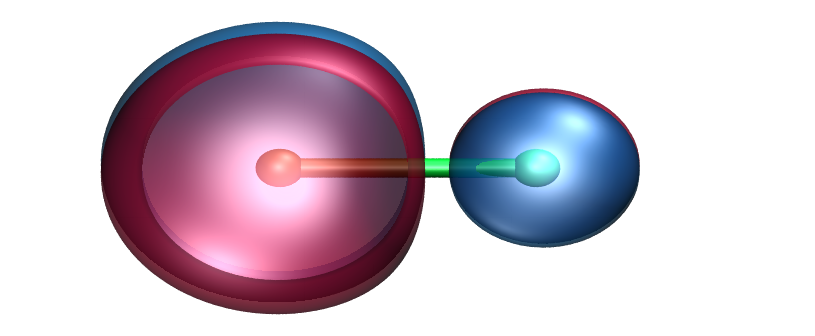
\includegraphics[height=0.6\textwidth]{Figures/lifr3_gs_mo7.cube.png}
        \caption*{\centering $(2\sigma_g)~n_\text{occ}~=~0.054$}
        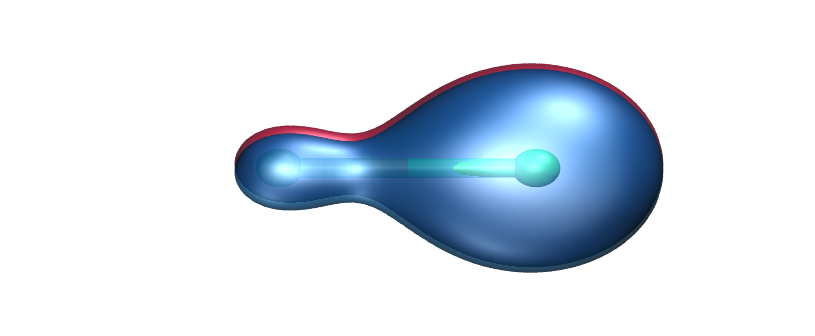
\includegraphics[height=0.6\textwidth]{Figures/lifr3_gs_mo6.cube.png}
        \caption*{\centering $(1\sigma_g)~n_\text{occ}~=~1.946$
        $E=-105.373~E_h$}
      \end{column}

      \begin{column}{0.31\textwidth}
        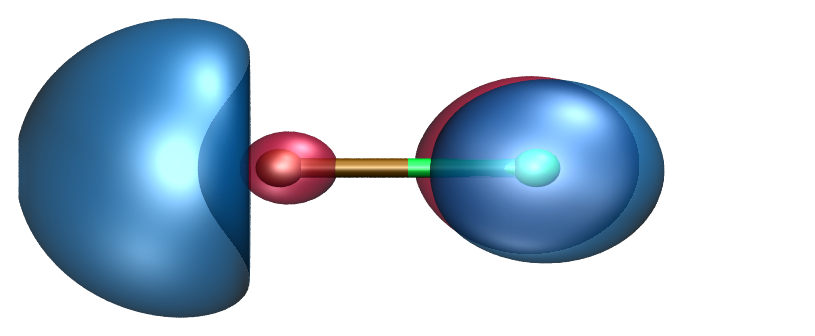
\includegraphics[height=0.6\textwidth]{Figures/lifr3_s1_mo7.cube.png}
        \caption*{\centering $(1\sigma_u)~n_\text{occ}~=~0.94162$}
        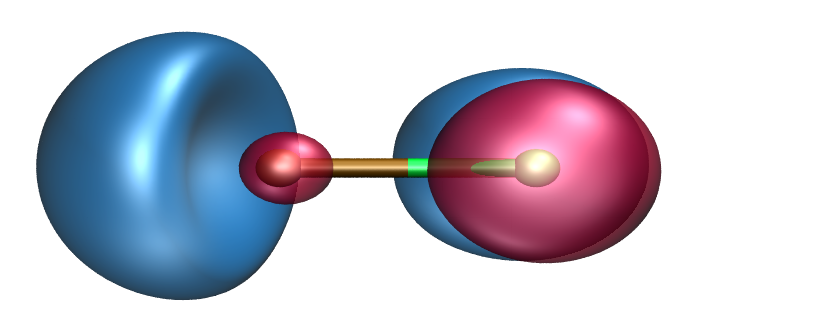
\includegraphics[height=0.6\textwidth]{Figures/lifr3_s1_mo6.cube.png}
        \caption*{\centering $(1\sigma_g)~n_\text{occ}~=~1.05838$
        $E=-105.317~E_h$}
      \end{column}

      \begin{column}{0.31\textwidth}
        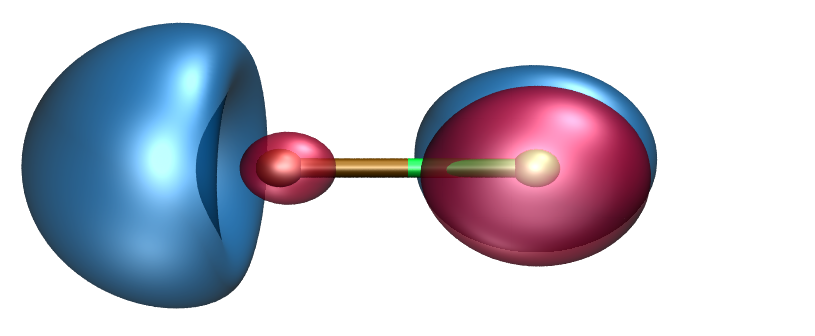
\includegraphics[height=0.6\textwidth]{Figures/lifr3_s2_mo7.cube.png}
        \caption*{\centering $(2\sigma_u)~n_\text{occ}~=~1.000$}
        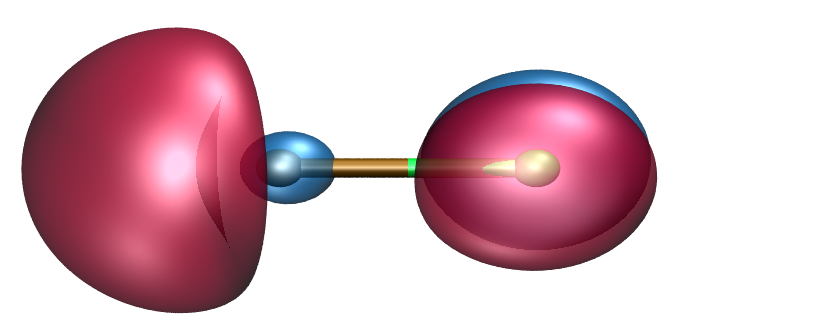
\includegraphics[height=0.6\textwidth]{Figures/lifr3_s2_mo6.cube.png}
        \caption*{\centering $(1\sigma_g)~n_\text{occ}~=~1.000$
        $E=-105.315~E_h$}
      \end{column}

    \end{columns}
  \end{figure}
\end{frame}

\begin{frame}{Natural orbitals of the three lowest singlet solutions: \ce{LiF} STO-3G}
  \begin{figure}
    \begin{columns}[b]
      
      \begin{column}{0.31\textwidth}
        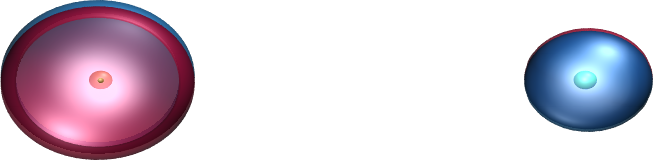
\includegraphics[width=0.9\textwidth]{Figures/lifr12_gs_mo7.cube.png}
        \caption*{\centering $(2\sigma_g)~n_\text{occ}~=~1.000$}
        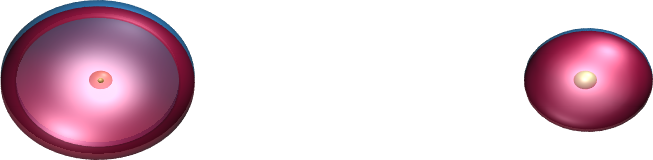
\includegraphics[width=0.9\textwidth]{Figures/lifr12_gs_mo6.cube.png}
        \caption*{\centering $(1\sigma_g)~n_\text{occ}~=~1.000$
        $E=-105.217~E_h$}
      \end{column}

      \begin{column}{0.31\textwidth}
        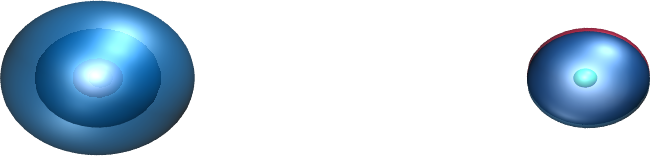
\includegraphics[width=0.9\textwidth]{Figures/lifr12_s1_mo7.cube.png}
        \caption*{\centering $(1\sigma_u)~n_\text{occ}~=~1.000$}
        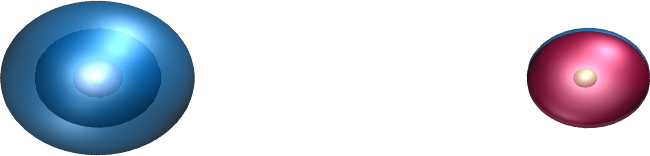
\includegraphics[width=0.9\textwidth]{Figures/lifr12_s1_mo6.cube.png}
        \caption*{\centering $(1\sigma_g)~n_\text{occ}~=~1.000$
        $E=-105.302~E_h$}
      \end{column}

      \begin{column}{0.31\textwidth}
        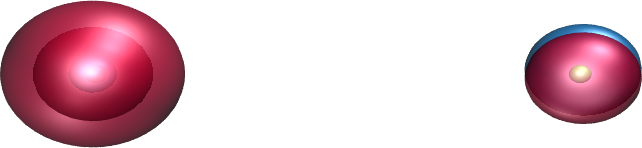
\includegraphics[width=0.9\textwidth]{Figures/lifr12_s2_mo7.cube.png}
        \caption*{\centering $(2\sigma_u)~n_\text{occ}~=~1.000$}
        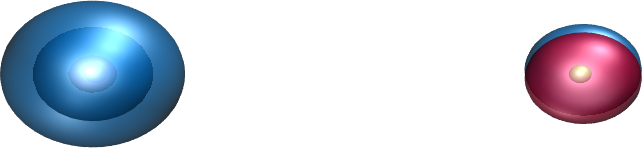
\includegraphics[width=0.9\textwidth]{Figures/lifr12_s2_mo6.cube.png}
        \caption*{\centering $(1\sigma_g)~n_\text{occ}~=~1.000$
        $E=-105.302~E_h$}
      \end{column}

    \end{columns}
  \end{figure}
\end{frame}

\begin{frame}{Strong avoided crossing: \ce{LiF} STO-3G}
  \begin{figure}
    \includegraphics<1>[width=0.9\textwidth]{Figures/fig_9c.pdf}
  \end{figure}
\end{frame}

\section{Conclusion}

\begin{frame}{Conclusion and open questions}
  \pause[1]
  \textbf{Results}
  \begin{itemize}[<+- | alert@+>]
  \item Origin of the CASSCF spurious solutions
  \item Lots of solutions but we understand them
  \item SS-CASSCF solutions behaves ``quasi-diabatically''
  \end{itemize}
  \pause[4]
  \textbf{Open questions}
  \begin{itemize}[<+- | alert@+>]
  \item LiF SS-CASSCF avoided crossing 
  \item Develop practical SS-CASSCF algorithms
  \item Which solutions these algorithms are converging toward?
  \end{itemize}
  \pause[7]
  \alert{Thanks to Hugh for supervising me!}
\end{frame}

\plain{Questions?}

\begin{frame}{Natural orbitals of the three lowest singlet solutions: \ce{LiF} STO-3G}
  \begin{figure}
    \begin{columns}[b]
      
      \begin{column}{0.31\textwidth}
        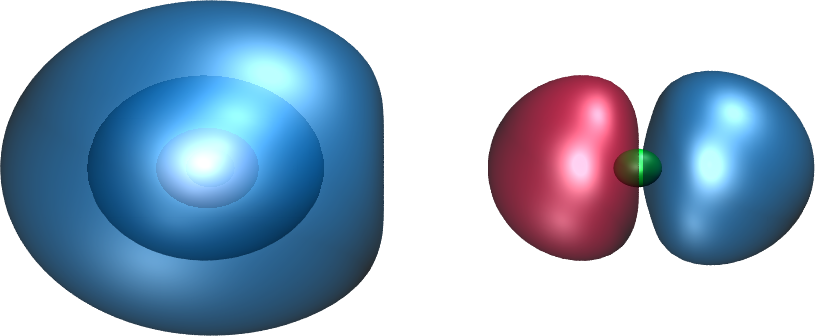
\includegraphics[width=0.9\textwidth]{Figures/lifr5_adiab_mo7.cube.png}
        \caption*{\centering $(2\sigma_g)~n_\text{occ}~=~0.566423$}
        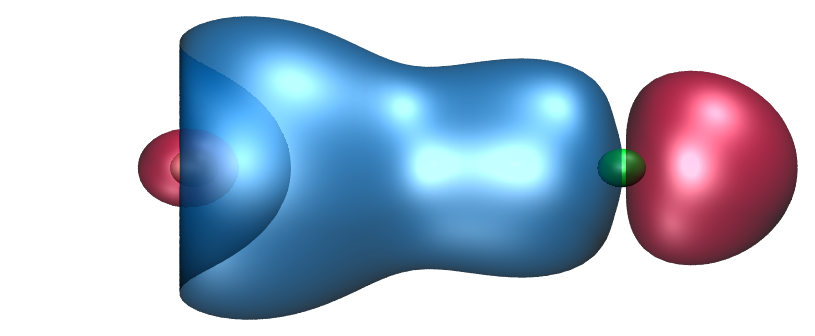
\includegraphics[width=0.9\textwidth]{Figures/lifr5_adiab_mo6.cube.png}
        \caption*{\centering $(1\sigma_g)~n_\text{occ}~=~1.43358$
        $E=-105.316~E_h$}
      \end{column}

      \begin{column}{0.31\textwidth}
        \includegraphics[width=0.9\textwidth]{Figures/lifr12_adiab_mo7.cube.png}
        \caption*{\centering $(1\sigma_u)~n_\text{occ}~=~0.997$}
        \includegraphics[width=0.9\textwidth]{Figures/lifr12_adiab_mo6.cube.png}
        \caption*{\centering $(1\sigma_g)~n_\text{occ}~=~1.003$
        $E=-105.302~E_h$}
      \end{column}

    \end{columns}
  \end{figure}
\end{frame}

\end{document}
